\documentclass[english,graybox,envcountchap,envcountsame,sectrefs,shortlabels]{svmono}
\usepackage{ifthen}
\newboolean{corrige}
%\setboolean{corrige}{true}  % <------------------ Le choix de société


\usepackage[T1]{fontenc}
\usepackage[latin9]{inputenc}
\usepackage[Lenny]{fncychap}
\usepackage{color}
\definecolor{page_backgroundcolor}{rgb}{1, 1, 1}
\pagecolor{page_backgroundcolor}
\definecolor{document_fontcolor}{rgb}{0, 0, 0}
\color{document_fontcolor}
\definecolor{shadecolor}{rgb}{1, 0, 0}
\usepackage{babel}
\usepackage{refstyle}
\usepackage{fancybox}
\usepackage{calc}
\usepackage{framed}
\usepackage{enumitem}
\usepackage{algorithm2e}
\usepackage{amsfonts, dsfont}
\usepackage{amsmath}
\let\proof\relax\let\endproof\relax
\usepackage{amsthm}
\usepackage{amssymb}
\usepackage{multicol,pdfsync}
\usepackage{makeidx}
\usepackage{minitoc}
\usepackage{xargs}
\usepackage{tikz}
\usepackage{hyperref}
\usetikzlibrary{automata}
\usetikzlibrary{patterns}

\makeindex
\usepackage{graphicx}
%\usepackage[unicode=true,
% bookmarks=false,
% breaklinks=false,pdfborder={0 0 1},backref=section,colorlinks=false]
% {hyperref}

\makeatletter



\newtheoremstyle{style}
  {6pt}% space above
  {30pt}% space below
  {\sffamily}%body font
  {-1em}%indent amount
  {\bfseries}%Theorem head
  {}%punctuation
  {1.5em}%space after theorem head
  {}

\theoremstyle{style}
\newtheorem{exo}{\textsc{Exercise}}

\newenvironment{answer}{\noindent \\ \textbf{Solution.}\begin{leftbar} \footnotesize}{\hfill \qed \end{leftbar}}

%\newtheoremstyle{styleQuestion}
%  {6pt}% space above
%  {6pt}% space below
%  {\sffamily}%body font
%  {13.5pt}%indent amount
%  {\sffamily}%Theorem head
%  {.}%punctuation
%  {0.5em}%space after theorem head
%  {}
%
%\ifthenelse{\boolean{corrige}}%
% {\theoremstyle{styleQuestion}%
% \newtheorem{question}{}}%
% {\theoremstyle{styleQuestion}%
% \newtheorem{question}{}}

\ifthenelse{\boolean{corrige}}%
   {}
   {\usepackage{environ}
   \NewEnviron{hide}{}
   \let\answer\hide
   \let\endanswer\endhide}

%%%%%%%%%%%%%%%%%%%%%%%%%%%%%% LyX specific LaTeX commands.

\AtBeginDocument{\providecommand\Eqref[1]{\ref{Eq:#1}}}
\AtBeginDocument{\renewcommand\eqref[1]{(\ref{#1})}}
\AtBeginDocument{\providecommand\Defref[1]{\ref{def:#1}}}
\AtBeginDocument{\providecommand\defref[1]{\ref{def:#1}}}
\AtBeginDocument{\providecommand\Lemref[1]{\ref{Lem:#1}}}
\AtBeginDocument{\providecommand\algref[1]{\ref{alg:#1}}}
\AtBeginDocument{\providecommand\Propref[1]{\ref{Prop:#1}}}
\AtBeginDocument{\providecommand\Thmref[1]{\ref{Thm:#1}}}
\AtBeginDocument{\providecommand\thmref[1]{\ref{thm:#1}}}
\AtBeginDocument{\providecommand\Corref[1]{\ref{Cor:#1}}}
\AtBeginDocument{\providecommand\Subsecref[1]{\ref{Subsec:#1}}}

\RS@ifundefined{subsecref}
  {\newref{subsec}{name = \RSsectxt}}
  {}
\RS@ifundefined{thmref}
  {\def\RSthmtxt{theorem~}\newref{thm}{name = \RSthmtxt}}
  {}
\RS@ifundefined{lemref}
  {\def\RSlemtxt{lemma~}\newref{lem}{name = \RSlemtxt}}
  {}


%%%%%%%%%%%%%%%%%%%%%%%%%%%%%% Textclass specific LaTeX commands.
\newenvironment{svmultproof}{\small \begin{proof}}{\end{proof}}
\renewenvironment{keywords}{\textit{\bf Keywords: } \sffamily }{}

%%%%%%%%%%%%%%%%%%%%%%%%%%%%%% User specified LaTeX commands.
\usepackage{a4wide,appendix,wrapfig}
\usepackage{bbm}
\definecolor{shadecolor}{RGB}{211,211,211}
\usepackage{pgf,framed}
%\renewenvironment{proof}%
%{\noindent \small {\textsc{Proof}.} \footnotesize}%
%{ \hfill$\blacksquare$\\}

\newenvironment{hyp}[1]{
\begin{enumerate}[label=(\textbf{\sf #1}\arabic*),resume=hyp#1]\begin{sf}}
{\end{sf}\end{enumerate}}



\global\long\def\defref#1{Definition~\ref{def:#1}}
\global\long\def\Defref#1{Definition~\ref{def:#1}}
\global\long\def\Lemref#1{Lemma~\ref{lem:#1}}
\global\long\def\Propref#1{Proposition~\ref{prop:#1}}
\global\long\def\Eqref#1{(\ref{eq:#1})}
\global\long\def\Thmref#1{Theorem~\ref{thm:#1}}
\global\long\def\lemref#1{Lemma~\ref{lem:#1}}
\global\long\def\propref#1{Proposition~\ref{prop:#1}}
\global\long\def\thmref#1{Theorem~\ref{thm:#1}}
\global\long\def\Subsecref#1{Section~\ref{subsec:#1}}
\global\long\def\Corref#1{Corollary~\ref{cor:#1}}
\global\long\def\algref#1{Algorithm~\ref{alg:#1}}


\newcommand{\iid}{\stackrel{\mathrm{i.i.d}}{\sim}}
\newcommandx{\dens}[3][1=,2=]%
{
\operatorname{p}_{#1}^{#2}(#3)
}
\newcommandx{\aslim}[1]{\ensuremath{\stackrel{#1 \mbox{-} \text{a.s.}}{\longrightarrow}}}
\newcommand{\Zset}{\mathsf{Z}}
\newcommand{\Zsigma}{\mathcal{Z}}
\newcommand{\borel}{\mathcal{B}}
\newcommand{\weaklim}{\ensuremath{\stackrel{\mathcal{L}_{\PP}}{\Rightarrow}}}
\newcommand{\eqLaw}{\stackrel{\mathcal L}{=}}
\newcommand{\indep}{\rotatebox[origin=c]{90}{$\models$}}
\newcommandx\functionsetspec[1][1=]{
\ifthenelse{\equal{#1}{c}}{\mathrm{C}}%fonctions continues
{\ifthenelse{\equal{#1}{bc}}{\mathrm{C}_b}%fonctions continues born\'{e}es
{\ifthenelse{\equal{#1}{u}}{\mathrm{U}}%fonctions uniform\'{e}ment continues
{\ifthenelse{\equal{#1}{bu}}{\mathrm{U}_b}%fonctions uniform\'{e}ment continues born\'{e}es
{\ifthenelse{\equal{#1}{l}}{\mathrm{Lip}}%fonctions lipschitz
{\ifthenelse{\equal{#1}{bl}}{\mathrm{Lip}_b}%fonctions lipschitz born\'{e}es
{\mathbb{F}_{#1}}%le reste
}}}}}}
\newcommandx\sequence[3][2=,3=]
{\ifthenelse{\equal{#3}{}}{\ensuremath{\{ #1_{#2}\}}}{\ensuremath{\{ #1_{#2}, \eqsp #2 \in #3 \}}}}
\newcommand{\Yset}{\mathsf{Y}}
\newcommand{\Ysigma}{\mathcal{Y}}
\newcommandx\dsequence[4][3=,4=]{\ensuremath{\{ (#1_{#3}, #2_{#3}), \eqsp #3 \in #4 \}}}
\newcommand{\Id}{\mathrm{I}}
\newcommand{\lrav}[1]{\left|#1 \right|}
\newcommand{\rme}{\mathrm{e}}
\newcommand{\rmi}{\mathrm{i}}
\newcommand{\fracc}[2]{\frac{#1}{#2}}
\newcommand{\bs}{\begin{shaded}}
\newcommand{\es}{\end{shaded}}
\newcommand{\bfr}{\begin{framed}}
\newcommand{\efr}{\end{framed}}
\newcommand{\blb}{\begin{leftbar}}
\newcommand{\elb}{\end{leftbar}}
\newcommand{\ltwo}{\mathrm{L}_2}
\newcommand{\dlim}[1]{\stackrel{\mathcal{L}_{#1}}{\Rightarrow}}
\newcommand{\plim}[1]{\stackrel{#1-prob}{\longrightarrow}}
\newcommand{\gauss}{\mathcal{N}}
\newcommand{\eqsp}{}
\newcommand{\xset}{\ensuremath{\mathsf{X}}}
\newcommand{\Xset}{\mathsf{X}}
\newcommand{\Xsigma}{\mathcal{X}}


\newcommand{\Uset}{\mathsf{U}}
\newcommand{\Usigma}{\mathcal{U}}
\makeatother

\providecommand{\corollaryname}{Corollary}
\providecommand{\definitionname}{Definition}
\providecommand{\examplename}{Example}
\providecommand{\exercisename}{Exercise}
\providecommand{\lemmaname}{Lemma}
\providecommand{\proofname}{Proof}
\providecommand{\propositionname}{Proposition}
\providecommand{\theoremname}{Theorem}

\begin{document}
\global\long\def\1{\mathbf{1}}%
\global\long\def\as{\PP-\mbox{a.s.}}%
\global\long\def\eqdef{:=}%
\global\long\def\eqlaw{\stackrel{\mathcal{L}}{=}}%
\global\long\def\funcset#1{\mathsf{F_{#1}}}%
\global\long\def\indi#1{\1_{#1}}%
\global\long\def\indiacc#1{\indi{\left\{  #1\right\}  }}%
\global\long\def\lfuncset#1{\mathsf{L_{#1}}}%
\global\long\def\lr#1{\left(#1\right)}%
\global\long\def\PE{\mathbb{E}}%
\global\long\def\lrb#1{\left[#1\right]}%
\global\long\def\lrcb#1{\left\{  #1\right\}  }%
\global\long\def\mcbb{\mathcal{B}}%
\global\long\def\meas#1{\mathsf{M}_{#1}}%
\global\long\def\mh#1{P_{\langle#1\rangle}^{MH}}%
\global\long\def\nset{\mathbb{N}}%
\global\long\def\mc#1{\mathcal{#1}}%
\global\long\def\mcf{\mathcal{F}}%
\global\long\def\mcg{\mathcal{G}}%
\global\long\def\PP{\mathbb{P}}%
\global\long\def\rmd{\mathrm{d}}%
\global\long\def\rset{\mathbb{R}}%
\global\long\def\seq#1#2{\lrcb{#1\,:\,#2}}%
\global\long\def\set#1#2{\lrcb{#1\,:\,#2}}%
\global\long\def\Xset{\mathsf{X}}%
\global\long\def\Xsigma{\mathcal{X}}%




\title{Introduction to computational statistics}
\author{Sylvain Le Corff}
%\subtitle{A crash course Monte Carlo methods for generative models
%\begin{figure}[!h]
%\centering
%\includegraphics[height=80pt]{hamilton.jpg}
%\includegraphics[height=80pt]{bayes.jpg}
%\includegraphics[height=80pt]{markov.jpg}
%\includegraphics[height=80pt]{ulam.jpg}
%\includegraphics[height=80pt]{metropolis.png}
%\includegraphics[height=80pt]{hastings.jpg}
%\end{figure}
%}
\date{}

\maketitle

\chapter{M-estimation Z-estimation, maximum likelihood}

\section{Method of moments}
Consider a measurable space $(\Omega,\mathcal{F})$ and i.i.d. random variables $(X_1,\ldots,X_n)$ taking values in a measurable space $(\Xset,\Xsigma)$. We assume that we have access to probabilities $(\mathbb{P}_\theta)_{\theta\in\Theta}$, where $\Theta \subset\rset^d$. For all $\theta\in\Theta$, we write $\mathbb{E}_\theta$ the expectation under $\mathbb{P}_\theta$ and $\mathbb{V}_\theta$ the variance. The objective is to estimate the unknown parameter $\theta\in\Theta$. The method of moments consists in choosing $d$ functions $T_j:\Xset\to \rset$, $1\leq j\leq d$, such that $\mathbb{E}_\theta[|T_j(X_1)|]<\infty$. Then, write for all $1\leq j \leq d$, $\theta\in\Theta$,
$$
e_j(\theta) = \mathbb{E}_\theta[T_j(X_1)]\eqsp.
$$
As the quantities $e_j(\theta)$, $1\leq j \leq d$, $\theta\in\Theta$,  are usually unknown, they may be estimated by using empirical estimates. Assuming that for $1\leq j\leq d$, $\mathbb{E}_\theta[|T_j(X_1)|^2]<\infty$, the Bienayme-Tchebychev inequality allows to quantify the empirical estimation error: for all $\varepsilon>0$,
$$
\mathbb{P}_\theta\left(\left|\frac{1}{n}\sum_{i=1}^{n}T_j(X_i)-e_j(\theta)\right|\geq \varepsilon\right) \leq \frac{\mathbb{V}_\theta[T_j(X_1)]}{n\varepsilon^2}\eqsp.
$$
In order to estimate the unknown parameter $\theta$ we may consider the system of equations:
$$
\forall j\in\{1,\ldots,d\},\quad e_j(\theta) = \frac{1}{n}\sum_{i=1}^n T_j(X_i)\eqsp.
$$
Assuming that this system has a unique solution $\widehat \theta_n$, $\widehat \theta_n$ is referred to as the moment estimator associated with $\{T_j\}_{1\leq j\leq d}$.

\begin{example}
Let $(X_1,\ldots,X_n)$ be i.i.d. random variables with exponential distribution with parameter $\theta>0$. Using $T_1:x\mapsto x$ and $T_2:x\mapsto x^2$ we have for all $\theta>0$,
$$
e_1(\theta) = \theta^{-1}\quad\mathrm{and}\quad e_2(\theta) = 2\theta^{-2}\eqsp.
$$
The moment estimator associated with $T_1$ is
$$
\widehat \theta_{n,1} = \frac{n}{\sum_{i=1}^nX_i}\eqsp.
$$
The moment estimator associated with $T_2$ is
$$
\widehat \theta_{n,2} = \left(\frac{2n}{\sum_{i=1}^nX^2_i}\right)^{1/2}\eqsp.
$$
\end{example}

\section{Z-estimation}
The moment estimator associated with $\{T_j\}_{1\leq j\leq d}$ is a solution to a system of equations of the form
$$
\frac{1}{n}\sum_{i=1}^n\psi(\theta,X_i) = 0\eqsp,
$$
where for all $\theta\in\Theta$, $x\in\Xset$,
$$
\psi(\theta,x)  =\begin{pmatrix}T_1(x) - \mathbb{E}_{\theta}[T_1(X_1)]\\ \vdots \\T_d(x) - \mathbb{E}_{\theta}[T_d(X_1)]\end{pmatrix}\eqsp.
$$
Consider now arbitrary functions $\psi_j$, $1\leq j\leq d$, such that for all $\theta_*\in\Theta$, $1\leq j \leq d$, $\mathbb{E}_{\theta_*}[|\psi_j(\theta_*,X_1)|]<\infty$. A Z-estimator associated with $\psi = (\psi_1,\ldots,\psi_d)^\top$ is any solution $\widehat\theta_n$ satisfying
$$
\psi_n(\widehat\theta_n) = 0\eqsp,
$$
where for all $\theta\in\Theta$,
$$
\psi_n(\theta) = \frac{1}{n}\sum_{i=1}^n\psi(\theta,X_i)\eqsp.
$$
\begin{example}
Let $F$ be a distribution function on $\mathbb{R}$ such that for all $x\in\mathbb{R}$, $F(x) = 1 - F(-x)$. Let $(X_1,\ldots,X_n)$ be i.i.d with distribution function $F_{\theta_*}$ where for all $\theta\in\mathbb{R}$, $x\in\mathbb{R}$, $F_\theta(x) = F(x-\theta)$. In this setting,
$$
\mathbb{E}_\theta[X_1] = \theta\eqsp,
$$
which suggests to choose $\psi(\theta,x) = x-\theta$. In this case, the Z-estimator associated with $\psi$ is given by $\widehat\theta_n = n^{-1}\sum_{i=1}^nX_i$.
\end{example}


\section{Maximum likelihood}
\begin{definition}
Let $(\Xset,\Xsigma)$ be a measurable space equipped with a sigma-finite measure $\mu$. Let $(f_\theta)_{\theta\in\Theta}$ be a family of probability densities with respect to $\mu$ and $(X_i)_{1\leq i\leq n}$ be i.i.d. random variables with probability density $f_{\theta_*}$, $\theta_*\in\Theta$. The likelihood of $(X_i)_{1\leq i\leq n}$ is the function
$$
L_n:\theta\mapsto \prod_{i=1}^nf_\theta(X_i)\eqsp.
$$
A maximum likelihood estimator associated with $L_n$ is any estimator solution to the following optimization problem
$$
\widehat\theta_n\in \mathrm{Argmax}_{\theta\in\Theta} L_n(\theta)\eqsp.
$$
\end{definition}

\begin{example}
Let $(X_i)_{1\leq i\leq n}$ be i.i.d. Bernoulli random variables with parameter $\theta_*\in(0,1)$. For all $\theta\in(0,1)$,
$$
L_n(\theta) = \prod_{i=1}^n \theta^{X_i}(1-\theta)^{1-X_i}
$$
and
$$
\ell_n(\theta) = \log L_n(\theta) = \left(\sum_{i=1}^nX_i\right)\log\theta + \left(\sum_{i=1}^n(1-X_i)\right)\log(1-\theta)\eqsp.
$$
The function $\ell_n/n$ is stricly concave on $(0,1)$ with $\lim_{\theta\to 0}\ell_n(\theta)/n  =-\infty$ and $\lim_{\theta\to 1}\ell_n(\theta)/n =-\infty$. This function has therefore a unique maximum given by
$$
\widehat\theta_n = \frac{1}{n}\sum_{i=1}^nX_i\eqsp.
$$
\end{example}

\section{M-estimation}
Maximum likelihood estimators are defined as solutions to optimization problems. This is the case of many estimation procedures. Consider for instance a function $m:\Theta\times \Xset \to \mathbb{R}$, $(\theta,x)\mapsto m_\theta(x)$, such that for all $\theta,\theta_*\in\Theta$, $\mathbb{E}_{\theta_*}[|m_\theta(X_1)|]<\infty$ and consider also $M_n:\theta\mapsto n^{-1}\sum_{i=1}^n m_\theta(X_i)$. For all $\delta>0$,
$$
\mathbb{P}_{\theta_*}\left(\left|M_n(\theta) - M_{\theta_*}(\theta)\right|\geq \delta\right)\leq \frac{\mathbb{V}_{\theta_*}[m_\theta(X_1)]}{n\delta^2}\eqsp,
$$
where
$$
M_{\theta_*}(\theta) = \mathbb{E}_{\theta_*}[m_\theta(X_1)]\eqsp.
$$
A M-estimator is any solution to the following optimization problem:
$$
\widehat\theta_n\in \mathrm{Argmax}_{\theta\in\Theta} M_n(\theta)\eqsp.
$$

\begin{example}
For all $1\leq k\leq n$, let $x_k\in\mathbb{R}^d$ and consider $(\xi_k)_{1\leq k\leq n}$  i.i.d. random variables with distribution $\mathcal{N}(0,1)$ and the linear regression model:
$$
Y_k = \sum_{\ell=0}^{p}\beta_\ell \varphi_\ell(x_k) + \sigma\varepsilon_k\eqsp,
$$
where $\theta = (\sigma,\beta)\in\mathbb{R}_+^*\times \mathbb{R}^{p+1}$. The joint density of the observations is:
$$
f_n:\theta\mapsto (2\pi\sigma^2)^{-n/2}\mathrm{exp}\left(-\frac{1}{2\sigma^2}\sum_{k=1}^n\left(Y_k-\sum_{\ell=0}^{p}\beta_\ell \varphi_\ell(x_k)\right)^2\right)\eqsp.
$$
The maximum likelihood estimator of $\beta$ coincides with the mean squared error estimator
$$
\widehat{\beta}_n \in\mathrm{Argmin}_{\beta\in \mathbb{R}^{p+1}} \sum_{k=1}^n\left(Y_k-\sum_{\ell=0}^{p}\beta_\ell \varphi_\ell(x_k)\right)^2\eqsp.
$$
Consider the matrix $\Phi$ in $\mathbb{R}^{n\times(p+1)}$ such that for all $1\leq i \leq n$, $1\leq j \leq p+1$, $\Phi_{i,j} = \varphi_{j-1}(x_i)$. Then, $\widehat{\beta}_n$ is solution to 
$$
\Phi\Phi^\top \widehat{\beta}_n = \Phi Y\eqsp,
$$
where $Y = (Y_1,\ldots,Y_n)^\top$.
\end{example}

\section{Consistency}

%\subsection*{M-estimation}
When for all $\theta,\theta_*$, $\mathbb{E}_{\theta_*}[|m_\theta(X_1)|]<\infty$, by the law of large numbers, in $\mathbb{P}_{\theta_*}$-probability,
$$
M_n(\theta) = \frac{1}{n}\sum_{i=1}^nm_\theta(X_i) \rightarrow_{n\to\infty} M_{\theta_*}(\theta) = \mathbb{E}_{\theta_*}[m_\theta(X_1)]\eqsp.
$$
We also assume that $\theta_*$ is a maximum of $M_{\theta_*}$.
\begin{theorem}
Consider the following assumptions.
\begin{itemize}
\item For all $\theta_*\in\Theta$, in  $\mathbb{P}_{\theta_*}$-probability, $\mathrm{sup}_{\theta\in\Theta}|M_n(\theta)-M_{\theta_*}(\theta)|\to_{n\to \infty} 0$.
\item For all $\theta_*\in\Theta$ and $\varepsilon>0$,
$$
\mathrm{sup}_{\theta\in\Theta; |\theta-\theta_*|>\varepsilon}M_{\theta_*}(\theta)<M_{\theta_*}(\theta_*)\eqsp.
$$
\item $(\widehat \theta_n)_{n\geq 0}$ is such that there exists $(\rho_n)_{n\geq 0}$ satisfying for all $\theta_*\in\Theta$,  in  $\mathbb{P}_{\theta_*}$-probability, $\rho_n \to_{n\to \infty} 0$ and
$$
\mathrm{liminf}_{n\to \infty} \mathbb{P}_{\theta_*}\left(M_n(\widehat \theta_n)\geq M_n(\theta_*) -\rho_n\right) =1\eqsp.
$$
Then, for all $\theta_*\in\Theta$,  in  $\mathbb{P}_{\theta_*}$-probability, $\widehat \theta_n \to \theta_*$.
\end{itemize}
\end{theorem}

\begin{proof}
For all $\theta_*\in\Theta$, since $\theta_*$ is a maximum of $M_{\theta_*}$,
\begin{align*}
0\leq M_{\theta_*}(\theta_*) - M_{\theta_*}(\widehat\theta_n)&\leq  M_{\theta_*}(\theta_*) - M_n(\theta_*) + M_n(\theta_*) - M_n(\widehat\theta_n) + M_n(\widehat\theta_n) - M_{\theta_*}(\widehat\theta_n)\\
&\leq 2 \mathrm{sup}_{\theta\in\Theta}|M_n(\theta)-M_{\theta_*}(\theta)|+ \rho_n \\
&\hspace{3cm} + \left\{M_n(\theta_*)-M_n(\widehat \theta_n)-\rho_n\right\}\mathds{1}_{M_n(\theta_*) - \rho_n>M_n(\widehat \theta_n)}\eqsp.
\end{align*}
Let $\varepsilon>0$. There exists $\eta>0$ such that $M_{\theta_*}(\theta)\leq M_{\theta_*}(\theta_*)-\eta$ for all $\theta\in\Theta$ such that $|\theta-\theta_*|\geq \varepsilon$. Therefore, $\{|\widehat\theta_n-\theta_*|\geq \varepsilon\}\subset\{M_{\theta_*}(\widehat\theta_n)\leq M_{\theta_*}(\theta_*)-\eta\}$. This yields 
$$
\mathbb{P}_{\theta_*}\left(|\widehat\theta_n-\theta_*|\geq \varepsilon\right)\leq \mathbb{P}_{\theta_*}\left(M_{\theta_*}(\widehat\theta_n)\leq M_{\theta_*}(\theta_*)-\eta\right) \leq \mathbb{P}_{\theta_*}\left(M_{\theta_*}(\theta_*) - M_{\theta_*}(\widehat\theta_n)>\eta\right) \eqsp,
$$
which concludes the proof.
\end{proof}

\begin{remark}
If $\Theta$ is compact in $\mathbb{R}^d$, $M_{\theta_*}$ is continuous, and for all $\theta\neq\theta_*$, $M_{\theta_*}(\theta)<M_{\theta_*}(\theta_*)$, the second assumption is satisfied.
\end{remark}

%\subsection*{Z-estimation}
\subsection{Exponential models}
Let $(X_1,\ldots,X_n)$ be i.i.d. random variables with density $p_{\theta_*}$ with respect to a reference measure $\mu$ on $(\mathbb{R}^d,\mathcal{B}(\mathbb{R}^d))$. The family $\{p_\theta\}_{\theta\in\Theta}$ is said to be in the exponential family if the rexist $\eta:\theta\to \mathbb{R}^d$, $T:\Xset\to\mathbb{R}^d$, $h:\Xset\to\mathbb{R}_+$, $B:\Theta\to\mathbb{R}$ such that for all $x\in\Xset$,
$$
p_\theta(x) = h(x)\exp\left(\langle \eta(\theta);T(x)\rangle - B(\theta)\right)\eqsp.
$$

\begin{example}
\begin{itemize}
\item The density of a Poisson distribution with parameter $\theta>0$ is given by
$$
p_\theta:x \mapsto \frac{\theta^x}{x!} \rme^{-\theta}\eqsp,
$$
so that $h(x) = (x!)^{-1}$, $T(x)=x$, $\eta(\theta) = \log \theta$, $B(\theta) = -\theta$.
\item If $\theta = (\mu,\sigma^2)\in\mathbb{R}\times\mathbb{R}_+^*$ and $p_\theta$ is the Gaussian probability density with mean $\mu$ and variance $\sigma^2$, $h(x) = 1$, $T(x)=(x,x^2)^\top$, $\eta(\theta) = (\mu/\sigma^2,-1/(2\sigma^2))^\top$, $B(\theta) = \log(2\pi\sigma^2)/2 + \mu/(2\sigma^2)$.
\end{itemize}
\end{example}
The canonical exponential family is given, for all $x\in\Xset$, by 
$$
p_\eta(x) = h(x)\exp\left(\langle \eta;T(x)\rangle - A(\eta)\right)\eqsp,
$$
where
$$
A(\eta) = \log\left(\int h(x)\exp\left(\langle \eta;T(x)\rangle \right)\mu(\rmd x)\right)\eqsp.
$$

\chapter{Expectation Maximization algorithm}

\section{Introduction}
Let $(\Uset,\Usigma)$ be a measurable space and $\lambda$ be a measure on $(\Uset,\Usigma)$. Consider also a family $\{f_\theta\}_{\theta\in\Theta}$ of $\lambda$-integrable and positive functions. Define
$$
L(\theta) = \int f_\theta(u)\lambda(\rmd u)\eqsp.
$$
We aim at solving
$$
\widehat \theta \in\mathrm{Argmax}_{\theta\in\Theta} L(\theta)\eqsp.
$$
When $L$ is positive, the problem is often written:
$$
\widehat \theta \in\mathrm{Argmax}_{\theta\in\Theta} \ell(\theta) = \log L(\theta)\eqsp.
$$

\begin{example}
\label{ex:EM}
A very popular setting is when  and $f_\theta: z \mapsto p_\theta(z,X)$ where $p_\theta$ is the joint probability density function of two random variables $(Z,X)$. Assuming that the random variable $X$ is observed and that $Z$ is not observed, we consider 
$$
L(\theta) = \int f_\theta(z,X)\lambda(\rmd z)\eqsp,
$$
which is a random variable depending on $X$. This is the marginal density of $X$ when the parameter is $\theta$. In this setting, $f_\theta(Z,X)/L(\theta)$ is the probability density of the conditional distribution of $Z$ given $X$.  Solving $\widehat \theta \in\mathrm{Argmax}_{\theta\in\Theta} L(\theta)$ amounts to solving the maximum likelihood estimation problem. However, in this setting, as in many other settings, the integral is intractable and the optimization problem cannot be solved directly.
\end{example}

\section{Algorithm}
In the following, we write $p_\theta:u\mapsto f_\theta(u)/L(\theta)$. Solving the optimization problem is not possible in general frameworks. The Expectation Maximization (EM) algorithm computes sequentially $\{\theta_k\}_{k\geq 0}$ to estimate $\widehat \theta$. For all $\theta,\theta'\in\Theta$, we introduce the following quantity:
$$
Q(\theta,\theta') = \int \log f_\theta(u)p_{\theta'}(u)\lambda(\rmd u) = \mathbb{E}_{\theta'}[\log f_\theta(U)]\eqsp,
$$
where $\mathbb{E}_{\theta}$ is a notation for the expectation under the density $p_\theta$. Then, we can write for all $\theta,\theta'\in\Theta$
$$
Q(\theta,\theta') = \int \log (L(\theta)p_\theta(u))p_{\theta'}(u)\lambda(\rmd u) = \ell(\theta) - H(\theta,\theta')\eqsp,
$$
where $H(\theta,\theta') = - \int \log p_\theta(u) p_{\theta'}(u)\lambda(\rmd u)$.

\begin{lemma}
\label{lem:fundEM}
For all $\theta,\theta'\in\Theta$,
$$
\ell(\theta)-\ell(\theta')\geq Q(\theta,\theta')-Q(\theta',\theta')\eqsp.
$$
\end{lemma}
\begin{proof}
By definition, for all $\theta,\theta'\in\Theta$,
\begin{align*}
Q(\theta,\theta')-Q(\theta',\theta') &= \ell(\theta)-\ell(\theta') + H(\theta',\theta') - H(\theta,\theta')\\
&= \ell(\theta)-\ell(\theta') + \int \log\left(\frac{p_\theta(u)}{p_{\theta'}(u)}\right)p_{\theta'}(u)\lambda(\rmd u)\eqsp.
\end{align*}
As $\log$ is concave, by Jensen's inequality, 
$$
\int \log\left(\frac{p_\theta(u)}{p_{\theta'}(u)}\right)p_{\theta'}(u)\lambda(\rmd u) \leq \log\int \frac{p_\theta(u)}{p_{\theta'}(u)}p_{\theta'}(u)\lambda(\rmd u) \leq 0\eqsp,
$$
which concludes the proof.
\end{proof}
By Lemma~\ref{lem:fundEM}, starting from a parameter estimate $\theta_k$, $k\geq 0$, a direct solution to obtain a parameter $\theta$ such that $\ell(\theta) \geq \ell(\theta_k)$ is to choose $\theta$ such that $Q(\theta,\theta_k)\geq Q(\theta_k,\theta_k)$. This result motivates the Expectation Maximization (EM) algorithm given in Algorithm~\ref{alg:EM} and introduced in \cite{}.

\begin{algorithm}
\caption{A generic EM algorithm}\label{alg:EM}
\KwData{Initial parameter estimate $\theta_0$}
\KwResult{A sequence of parameter estimate $\{\theta_k\}_{k\geq 0}$}
\For{$k \geq 0$}{
  Compute the E-step: $\theta\mapsto Q(\theta,\theta_k)$\;
 Compute the M-step: $\theta_{k+1}\in \mathrm{Argmax}_{\theta\in\Theta}Q(\theta,\theta_k)$\;
}
\end{algorithm}

The most common setting in which the EM algorithm is used is the case of Example~\ref{ex:EM}. 

\begin{example}
\label{ex:EM:alg}
In the setting of Example~\ref{ex:EM:alg}, we have
$$
Q(\theta,\theta') = \int \log p_\theta(z,X)p_{\theta'}(z|X)\lambda(\rmd z) = \mathbb{E}_{\theta'}[\log p_\theta(Z,X)|X]\eqsp.
$$
Therefore, the E-step of the EM algorithm amounts to computing the conditional expectation given $X$ of the complete data (joint) loglikelihood.
\end{example}

\chapter{Variatonal inference and autoencoders}


\section*{Evidence Lower Bound}
In this chapter, we consider models with latent (unobserved) data. Let $(Z,X)$ be random variables in $\mathbb{R}^d\times \mathbb{R}^m$. We assume that the law of $(Z,X)$ has a density $(z,x)\mapsto p(z,x)$ with respect to a reference measure. In this setting, we write
$$
(z,x)\mapsto p(z,x) = p(z)p(x|z)\,,
$$
where $z\mapsto p(z)$ is a prior density for $Z$ and $x \mapsto p(x|z)$ is a conditional density (likelihood) of $X$ given $Z$. We do not have access to the conditional density of $Z$ given $X$, since this density is given by:
$$
z\mapsto p(z|x) = \frac{p(z)p(x|z)}{p(x)}\propto p(z)p(x|z)\,, 
$$
where $p(x) = \int p(z)p(x|z) \mathrm{d} z$ is an intractable integral.

\medskip

In variational inference, we introduce a variational family i.e. a family of densities to  approximate $z\mapsto p(z|x)$. Let $\mathcal{D}$ be such a family, where the densities $q \in\mathcal{D}$ satisfy the two following assumptions.
\begin{itemize}
\item For all $q\in \mathcal{D}$, $q$ is easy to evaluate.
\item For all $q\in \mathcal{D}$, $q$ is easy to sample from.
\end{itemize}

\medskip

Then, for all $x$ and all $q\in \mathcal{D}$, writing $\mathrm{KL}$ the Kullback-Leibler divergence between two probability distributions,
\begin{align*}
\mathrm{KL}\left(q\|p(\cdot|x)\right) = \int q(z) \log \frac{q(z)}{p(z|x)} \mathrm{d}z&= \mathbb{E}_{q}[\log q(Z)] - \mathbb{E}_{q}[\log p(Z|x)]\,,\\
 &= \mathbb{E}_{q}[\log q(Z)] - \mathbb{E}_{q}[\log p(Z,x)]+\log p(x)\,,\\
&= -\mathrm{ELBO}(q)+\log p(x)\,,
\end{align*}
where
$$
\mathrm{ELBO}(q) = \mathbb{E}_{q}\left[\log \frac{p(Z,x)}{q(Z)}\right]\,.
$$
Using Jensen's inequality, we obtain $\mathrm{KL}\left(q_\phi\|p(\cdot|x)\right) \geq 0$ so that
$$
\mathrm{ELBO}(q)\leq \log p(x)\,.
$$
This inequality justifies the name Evidence Lower BOund for $\mathbb{E}_{q}[\log (p(Z,x)/q(Z))]$. In variational inference, we then aim to approximate  $p(\cdot|x)$ by $q_{*}$ where :
$$
q_* \in \mathrm{argmax}_{q\in \mathcal{D}}\;\mathrm{ELBO}(q)\,.
$$

\section*{Coordinate ascent variational inference}
The most straightforward approach to solve the optimization problem is to consider a mean-field variational family  i.e. to choose $\mathcal{D}$ such that: 
$$
\mathcal{D} = \left\{z\mapsto q(z) = \prod_{j=1}^dq_j(z_j)\;;\; q_j \,\mbox{is\, a\, density} \right\}\,.
$$
In this case, we can write, for all $q\in \mathcal{D}$, and all $j\in\{1,\ldots,d\}$,
\begin{align*}
\mathrm{ELBO}(q) &= \mathbb{E}_{q}\left[\log \frac{p(Z_1,\ldots,Z_d,x)}{\prod_{j=1}^dq_j(Z_j)}\right]\,,\\
&= \mathbb{E}_{q_j}\left[\mathbb{E}_{q_{-j}}\left[\log p(Z_j | Z_{-j},x)\right]\right] - \mathbb{E}_{q_j}\left[\log q_j(Z_j)\right]  + \mathrm{cste}
\end{align*}
where $\mathrm{cste}$ does not depend on $q_j$,  $z_{-j} = (z_\ell)_{1\leq \ell \leq d; \ell \neq j}$ and $q_{-j}(z_{-j}) = \prod_{1\leq \ell \leq d; \ell \neq j}q_{\ell}(z_{\ell})$. 

\medskip

Assume that we want to optimize $\mathrm{ELBO}(q) $ on $q_j$ only, the other densities $(q_\ell)_{\ell\neq j}$ being kept fixed. Consider the density $\tilde q_j$ such that
$$
\tilde q_j(z_j) \propto \exp\left(\mathbb{E}_{q_{-j}}\left[\log p(z_j | Z_{-j},x)\right]\right)\,,
$$
i.e. the desnity given by $\tilde q_j(z_j)= \exp(\mathbb{E}_{q_{-j}}[\log p(z_j | Z_{-j},x)])/C_j$ where $C_j$ does not depend on $z_j$. Therefore,
$$
\mathrm{ELBO}(q) = -\mathbb{E}_{q_j}\left[\log \frac{q_j(Z_j)}{\tilde q_j(Z_j) }\right]  + \mathrm{cste} + \log C_j = -\mathrm{KL}(q_j\|\tilde q_j)  + \mathrm{cste} + \log C_j\,.
$$
Therefore, optimizing  $\mathrm{ELBO}(q) $ on $q_j$ only, the other densities $(q_\ell)_{\ell\neq j}$ being kept fixed, yields an optimum given by $\tilde q_j$.
The algorithm Coordinate Ascent Variational Inference (CAVI) proposes therefore to sequentially update  $q_j$, $1\leq j \leq d$ until a stopping criterion is met. In Algorithm~\ref{alg:CAVI}, we propose a version of the algorithm where the variational distribution of only one component of $Z$ is updated at each iteration, of course many alternatives can be considered. A standard alternative is to update each variational distribution at each iteration.

\begin{algorithm}[H] \label{alg:CAVI}
    \KwData{Observation $x$, mean-field family $\mathcal{D}$, initial variational distribution $\{q_j^{(0)}\}_{1\leq j \leq d}$, maximum number of iteration $N$}
    \KwResult{A variational distribution for each coordinate of $Z$, $q^{(N)}_j$, $1\leq j\leq d$.}
    \For {$ k= 1 \to N$}{
        Draw $j\in\{1,\ldots,d\}$ uniformly at random;

        Set $q^{(k)}_\ell = q^{(k-1)}_\ell$ for all $1\leq \ell \leq d$, $\ell \neq j$ and $q^{(k)}_{-j} = \prod_{1\leq \ell \leq d, \ell\neq j} q^{(k)}_{\ell}$;

        Set $$q^{(k)}_j(z_j) \propto \exp\left(\mathbb{E}_{q_{-j}^{(k)}}\left[\log p(z_j | Z_{-j},x)\right]\right)$$;
}
\end{algorithm}

\section*{Application to a mixture of Gaussian distributions}
Consider a mixture of $K$ Gaussian distributions with means $\mu = (\mu_k)_{1\leqslant k \leqslant K}$ and variance 1. The variables  $\mu = (\mu_k)_{1\leqslant k \leqslant K}$ are  i.i.d. Gaussian with mean 0 and variance $\sigma^2$. For all $1\leq i\leq n$, we denote by $c_i\in\{1\leq i \leq K\}$ the group $X_i$ belongs to, this variable is not observed. The weight of component  $k$ is written $\omega_k$, i.e. conditionally on $\mu$, $c= (c_i)_{1\leq i\leq n}$ are independent with multinomial distribution with parameters $\{\omega_1,\ldots,\omega_K\}$ (in particular, $c$ is independent of $\mu$).  

Conditionally on  $\mu$ and $c$, the observations $(X_i)_{1\leqslant i\leqslant n}$ are i.i.d., and $X_i$ has a Gaussian distribution with mean $\mu_{c_i}$ and variance $1$. Marginalizing on $c$, conditionally on  $\mu$, the observations $(X_i)_{1\leqslant i\leqslant n}$ are i.i.d. and the conditional probability density of $X_1$ is:
$$
x\mapsto p(x|\mu,\omega) = \sum_{k=1}^K \omega_k \varphi_{\mu_k,1}(x)\,,
$$
where $\varphi_{\mu_k,\eta^2}$ the Gaussian probability density function with mean $\mu_k$ and  variance $\eta^2$. The joint likelihood is therefore:
$$
p(x_1,\cdots,x_n) = \int p(x_1,\cdots,x_n|\mu) p(\mu) \mathrm{d} \mu = \int \prod_{i=1}^n p(x_i|\mu) p(\mu) \mathrm{d} \mu = \int \prod_{i=1}^n \left(\sum_{k=1}^K \omega_k \varphi_{\mu_k,1}(x_i)\right) p(\mu) \mathrm{d} \mu
$$
Writing $z = (\mu,c)$, our objective is to estimate $p(\mu,c|x)$ where $c = (c_1,\cdots,c_n)$ are the components of the observations. The  `mean-field` approximation writes:
$$
q(\mu,c) = \prod_{k=1}^K \varphi_{m_k,s_k}(\mu_k)\prod_{i=1}^n \mathrm{Cat}_{\phi_i}(c_i)\,, 
$$
which means that under $q$:
\begin{itemize}
\item $\mu$ and  $c$ are independent.
\item $(\mu_{k})_{1\leqslant k \leqslant K}$ are independent Gaussian random variables with means $(m_{k})_{1\leqslant k \leqslant K}$ and variances $(s_{k})_{1\leqslant k \leqslant K}$.
\item $(c_{i})_{1\leqslant i \leqslant n}$ are independent with  multinomial distributions with parameters  $(\phi_i)_{1\leqslant i \leqslant n}$: $q(c_i=k) = \phi_i(k)$ for $1\leqslant k \leqslant K$. 
\end{itemize}
Write $\mathcal{D}$ this family where the means $(m_{k})_{1\leqslant k \leqslant K}\in \mathbb{R}^K$, and variances $(s_{k})_{1\leqslant k \leqslant K}\in (\mathbb{R}_+^*)^K$ and the parameters  $(\phi_i)_{1\leqslant i \leqslant n}\in \mathcal{S}_K^n$ where $\mathcal{S}_K$ is the simplex of dimension $K$.  Then, we aim at solving the optimization problem:
$$
q^* = \mathrm{Argmin}_{q\in\mathcal{D}}\; \mathrm{KL}\left(q\|p(\cdot|x)\right)\,.
$$
Note that
\begin{align*}
\mathrm{KL}\left(q\|p(\cdot|x)\right) &= \mathbb{E}_q[\log q(\mu,c)] - \mathbb{E}_q[\log p(\mu,c|x)]\,,\\
 &= \mathbb{E}_q[\log q(\mu,c)] - \mathbb{E}_q[\log p(\mu,c,x)]+\log p(x)\,,\\
&= -\mathrm{ELBO}(q)+\log p(x)\,,
\end{align*}
where
$$
\mathrm{ELBO}(q) = -\mathbb{E}_q[\log q(\mu,c)] + \mathbb{E}_q[\log p(\mu,c,x)] \,.
$$
CAVI algorithm computes iteratively $1\leqslant k \leqslant K$,
$$
q(\mu_k) \propto \mathrm{exp}\left(\mathbb{E}_{\tilde q_{\mu_k}}[\log \tilde p_k(\mu_k|x)]\right)
$$
and for all $1\leqslant i \leqslant n$,
$$
q(c_i) \propto \mathrm{exp}\left(\mathbb{E}_{\tilde q_{c_i}}[\log \tilde p_i(c_i|x)]\right)\,,
$$
where
\begin{itemize}
\item $\tilde p_i(c_i|x)$ is the conditional distribution of $c_i$ given the observations and the other parameters  and $\tilde p_k(\mu_k|x)$ is the conditional distribution of $\mu_k$ given the observations and the other parameters.
\item $\mathbb{E}_{\tilde q_z}$ is the expectation under the variational distribution of all variables except $z$.
\end{itemize}
Note that
$$
\tilde p_i(c_i|x) \propto p(c_i)p(x_i|c_i,\mu) \propto p(c_i)\prod_{k=1}^K \left(\varphi_{\mu_k,1}(x_i)\right)^{1_{c_i=k}}\,. 
$$
Then,
$$
\mathbb{E}_{\tilde q_{c_i}}[\log \tilde p_i(c_i|x)] = \log p(c_i) + \sum_{k=1}^K 1_{c_i=k} \mathbb{E}_{\tilde q_{c_i}}[\log \varphi_{\mu_k,1}(x_i)]
$$
and
\begin{align*}
\mathrm{exp}\left(\mathbb{E}_{\tilde q_{c_i}}[\log \tilde p_i(c_i|x)]\right) &\propto p(c_i) \mathrm{exp}\left(\sum_{k=1}^K 1_{c_i=k} \mathbb{E}_{\tilde q_{c_i}}[\log \varphi_{\mu_k,1}(x_i)]\right)\,\\
&\propto p(c_i) \mathrm{exp}\left(\sum_{k=1}^K 1_{c_i=k} \mathbb{E}_{\tilde q_{c_i}}[-(x_i-\mu_k)^2/2]\right)\,\\
&\propto p(c_i) \mathrm{exp}\left(\sum_{k=1}^K 1_{c_i=k} \mathbb{E}_{\tilde q_{c_i}}[-(x_i-\mu_k)^2/2]\right)\,.
\end{align*}
The update writes :
$$
\varphi_i(k) \propto p(c_i=k) \mathrm{exp}\left(m_k x_i - \frac{m^2_k + s_k}{2}\right)\,.
$$
Since $\tilde p_k(\mu_k|x)$ is the conditional law of $\mu_k$ given the observations and the other parameters,
$$
\tilde p_k(\mu_k|x) \propto p(\mu_k)\prod_{i=1}^np(x_i|c_i,\mu) \,. 
$$
Then,
$$
\mathbb{E}_{\tilde q_{\mu_k}}[\log \tilde p_k(\mu_k|x)] = \log p(\mu_k) + \sum_{i=1}^n \mathbb{E}_{\tilde q_{\mu_k}}[\log p(x_i|\mu,c_i)]
$$
and
\begin{align*}
\mathrm{exp}\left(\mathbb{E}_{\tilde q_{\mu_k}}[\log \tilde p_i(c_i|x)]\right) &\propto p(\mu_k) \mathrm{exp}\left(\sum_{i=1}^n\sum_{k=1}^K  \mathbb{E}_{\tilde q_{\mu_k}}[1_{c_i=k}\log \varphi_{\mu_k,1}(x_i)]\right)\,\\
&\propto p(\mu_k) \mathrm{exp}\left(\sum_{i=1}^n \phi_i(k) \mathbb{E}_{\tilde q_{\mu_k}}[\log \varphi_{\mu_k,1}(x_i)]\right)\,\\
&\propto \mathrm{exp}\left(-\frac{\mu_k^2}{2\sigma^2}-\frac{1}{2}\sum_{i=1}^n \phi_i(k)(x_i-\mu_k)^2\right)\,,\\
&\propto \mathrm{exp}\left(-\frac{\mu_k^2}{2\sigma^2}+\sum_{i=1}^n \phi_i(k)x_i\mu_k - \frac{1}{2}\sum_{i=1}^n \phi_i(k)\mu^2_k\right)\,.
\end{align*}
The update writes therefore,
$$
\mu_k = \frac{\sum_{i=1}^n \phi_i(k)x_i}{1/\sigma^2 + \sum_{i=1}^n \phi_i(k)}\quad\mathrm{and}\quad s_k = \frac{1}{1/\sigma^2 + \sum_{i=1}^n \phi_i(k)}\,. 
$$

\section*{Variational Autoencoders}
Variational Auto-Encoders (VAE) are very popular approaches to introduce approximations of a target conditional distribution in the context of latent data models. We consider a family of joint probability distributions $\{(z,x) \mapsto  p_{\theta}(z,x)\}_{\theta\in\Theta}$ on $(\mathsf{Z}\times \mathsf{X}, \mathcal{Z}\times \mathcal{X})$ where $Z$ is a latent variable and $X$ is the observation. In this setting, we often write, for all $\theta$, $x$, $z$,
$$
p_{\theta}(z,x) = p_{\theta}(z)p_{\theta}(x|z)
$$
and the conditional distribution $p_{\theta}(z|x)$ is not availbale explicitly. This setting is similar to the variational framework presented before but we also want to optimize the parameter $\theta$.

A variational approach can be introduced in this setting by considering a family $\{(z,x) \mapsto q_{\varphi}(z|x)\}_{\varphi\in\Phi}$ where $\Phi$ is a parameter space. Then, we can write, for all $\varphi,\theta$, $x$, $z$,
\begin{multline*}
\log p_\theta(x) = \int p_\theta(x) q_{\varphi}(z|x) \rmd z = \mathbb{E}_{q_{\varphi}(\cdot|x)}\left[\log p_\theta(x)\right] = \mathbb{E}_{q_{\varphi}(\cdot|x)}\left[\log \frac{p_\theta(Z,x)}{p_\theta(Z|x)}\right] \\
= \mathbb{E}_{q_{\varphi}(\cdot|x)}\left[\log \frac{q_{\varphi}(Z|x)}{p_\theta(Z|x)}\right]  + \mathbb{E}_{q_{\varphi}(\cdot|x)}\left[\log \frac{p_\theta(Z,x)}{q_{\varphi}(Z|x)}\right] .
\end{multline*}
The first term of the right-hand-side is the Kullback-Leibler divergence between $q_{\varphi}(\cdot|x)$ and $p_\theta(\cdot|x)$, so that $\log p_\theta(x)\geq \mathcal{L}(\theta,\varphi,x)$, where
$$
\mathcal{L}(\theta,\varphi,x) = \mathbb{E}_{q_{\varphi}(\cdot|x)}\left[\log \frac{p_\theta(Z,x)}{q_{\varphi}(Z|x)}\right]
$$
is the ELBO in this setting. Assuming that we have a dataset with i.i.d. data $\{x_i\}_{1\leq i \leq n}$, VAE propose to solve the optimization problem:
$$
(\widehat \varphi_n,\widehat \theta_n) \in \mathrm{argmin}_{\varphi\in\Phi,\theta\in\Theta} \frac{1}{n}\sum_{i=1}^n\mathcal{L}(\theta,\varphi,x_i).
$$
Of course, the joint optimization of $\theta$ and $\varphi$ is a complex problem both for practical and theoretical reasons and many research works have been devoted to this problem in the past few years. Solving this optimization problem aims at finding a parameter $\theta$ solving the maximum likelihood estimation problem and a paramter $\varphi$ such that $q_{\varphi}(\cdot|x)$ is a good approximation of $p_{\theta}(\cdot|x)$

In practice, the optimization problem is solved using a gradient descent algorithm using mini-batches of observations and Monte Carlo estimates of the expectations under $q_{\varphi}(\cdot|x)$.

\begin{figure}
\centering
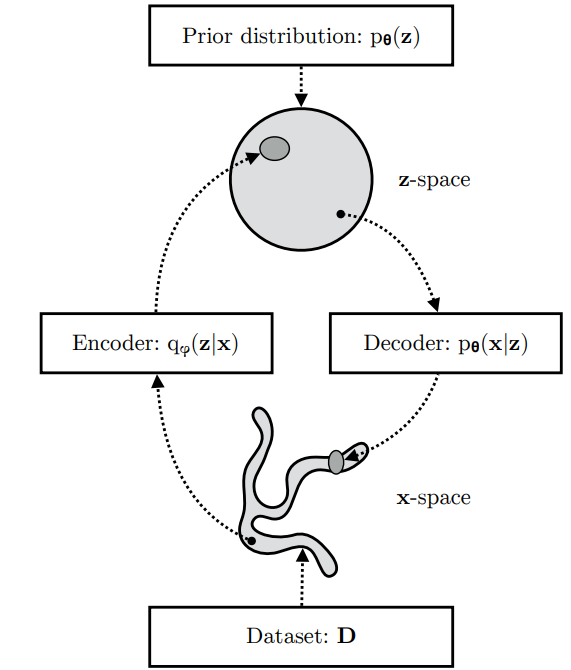
\includegraphics[scale=0.8]{vae.png}
\caption{An illustration of a VAE. From "An Introduction to Variational Autoencoders", Kingma et al., 2019.}
\label{fig:vae}
\end{figure}

\chapter{Markov chain Monte Carlo}

\section{Introduction}
This chapter aims at designing algorithms to obtain samples from a complex distribution $\pi$ defined on a measurable space $(\mathsf{X},\mathcal{X})$. Such algorithms can be applied in many situations, the target distribution $\pi$ can have several forms depending on the different contexts. The target distribution can be given for instance by a marginal density $p_\theta(y) = \int p_\theta(x,y) \lambda(\rmd x)$ or by a conditional/posterior distribution $p_\theta(x|y) = p_\theta(x)p_\theta(y|x)/\int p_\theta(x,y) \lambda(\rmd x)$ where $\theta\in\Theta$ and $\lambda$ is a dominating measure.

 %In this section, we introduce different algorithms, depending on the framework, to solve machine learning tasks based on sampling random variables.  In particular, we detail Markov Chain Monte Carlo (MCMC) methods, which allow to construct a process $(X_k)_{k\in\nset}$ that targets an unknown distribution $\pi$. Sometimes $(X_k)_{k\in\nset}$ is itself a Markov chain with invariant probatility measure $\pi$, sometimes, $(X_k)_{k\in\nset}$ is the first component process of an extended Markov chain that targets an extended distribution where the marginal distribution on the first component is $\pi$.

\begin{example}
%\paragraph{Bayesian inference. }
In  Bayesian inference, prior belief  is combined with
data to obtain posterior distributions on which statistical inference is based.
%Although we focus primarily on  likelihood based inference in this text,
%it is also worthwhile to consider Bayesian  inference  for some problems.
Except for some simple cases, Bayesian inference can be computationally
intensive and may rely on  computational techniques.


The basic idea in Bayesian analysis is that a parameter vector $ \theta \in \Theta$ is unknown, so it is endowed with a \emph{prior} distribution with probability density
$\pi_0( \theta)$.  We also
introduce a model or likelihood, $\dens[][]{ y_{1:n} \mid \theta}$, that is
a probability density function for the data $y_{1:n}$ which depends on the parameter vector.
Inference about $ \theta$ is then based on the \emph{posterior}
distribution, which is obtained via Bayes's theorem,
$$
\theta \mapsto \pi(\theta) =\frac{\pi_0( \theta) \dens[][]{ y_{1:n} \mid \theta}}{\int \pi_0( \theta) \dens[][]{ y_{1:n} \mid \theta} \lambda(\rmd \theta)} \propto \pi_0( \theta) \dens[][]{ y_{1:n} \mid \theta}.
$$
  In some simple cases, the prior  and
the likelihood are \emph{conjugate}  distributions that may be combined easily.
For example, in $n$ fixed repeated (i.i.d.) Bernoulli experiments with probability of success $\theta$,
a \emph{Beta-Binomial} conjugate pair is taken.  In this case the prior is
Beta($a,b$):
$\pi_0(\theta) \propto \theta^{a} (1-\theta)^{b}\mathds{1}_{(0,1)}(\theta)$; the values $a,b > -1$  are called
hyperparameters. The likelihood in this example is
Binomial$(n,\theta)$:
$\dens[][]{ y \mid \theta} \propto \theta^y (1-\theta)^{n-y}$, from which
we easily deduce that the
posterior is also Beta,
$\pi ( \theta ) \propto \theta^{y+a}(1-\theta)^{n+b-y }\mathds{1}_{(0,1)}(\theta)
$, and from which inference may easily be achieved.

In more complex experiments, the posterior distribution is often difficult to obtain by direct calculation,
so alternatives have to be deployed to obtain samples approximately distributed as the posterior distribution. 
\end{example}
%Note that in \eqref{eq:target:bayes}, the numerator is usually known and explicit while, due to the integral, the denominator is a multiplicative unknown constant.  

\begin{example}
Energy-based models (EBM) are very flexible models which describe the target distribution using an unnormalized function, referred to as the energy function. These models are easier to design that models with a tractable likelihood such as autoregressive models, in particular in high-dimensional setting. As the energy function is not normalized, it can
be easily parameterized with any nonlinear regression function. Using neural networks such as Multi-layer Perceptrons, or convolutional neural networks, is it straightforward to introduce energy function with specific structures depending nonlinearly on the input. %We can choose specific
%architectures tailored for every type of data, see \cite{song2021train} for a recent overview of EBM.

In a generic setting, the target random variable take values in $(\rset^d,\mathcal{B}(\rset^d))$ and the target distribution (the target density with respect to the Lebesgue measure) is written:
$$
x\mapsto \pi_\theta(x) \propto \exp\left(-\mathrm{E}_\theta(x)\right) = \frac{\exp\left(-\mathrm{E}_\theta(x)\right)}{\int \exp\left(-\mathrm{E}_\theta(u)\right)\rmd u},
$$
where $\theta$ is an unknown parameter to estimate and $\mathrm{E}_\theta$ is the energy function. The normalizing constant is often written $Z_\theta$ and referred to as the partition function:
$$
Z_\theta = \int \exp\left(-\mathrm{E}_\theta(u)\right)\rmd u.
$$
Since $Z_\theta$ is an intractable integral, evaluation and
differentiation of $x\mapsto \log \pi_\theta(x)$ is not possible in usual settings. In order to estimate the unknwon parameter $\theta$ using i.i.d. data an appealing approach is to use gradient-based maximization procedure of the likelihood function. This means that we need to compute:
$$
x\mapsto \nabla_\theta \log\pi_\theta(x) = -\nabla_\theta\mathrm{E}_\theta(x) - \nabla_\theta \log Z_\theta.
$$
The first term can be evaluated easily as $\mathrm{E}_\theta(x)$ is known. For the second term, we can write, under regularity assumptions on the model:
\begin{multline*}
\nabla_\theta \log Z_\theta = Z_\theta^{-1} \int \nabla_\theta\exp\left(-\mathrm{E}_\theta(u)\right)\rmd u \\=  \int \left\{-\nabla_\theta \mathrm{E}_\theta(u)\right\}Z_\theta^{-1}\exp\left(-\mathrm{E}_\theta(u)\right)\rmd u = \int \left\{-\nabla_\theta \mathrm{E}_\theta(u)\right\}\pi_\theta(u)\rmd u .
\end{multline*}
Therefore $\nabla_\theta \log Z_\theta = \mathbb{E}_{\pi_\theta}[-\nabla_\theta \mathrm{E}_\theta(X)]$ where $\mathbb{E}_{\mu}[f(X)]$ denotes the expectation of $f(X)$ when $X\sim \mu$. Therefore, it is possible to train an EBM by providing a Monte Carlo estimate of $\nabla_\theta \log Z_\theta$ which requires to obtain samples from $\pi_\theta$. However, this is not straightforward as $\pi_\theta$ is known only up to a multiplicative normalizing constant (as in the Bayesian setting).
\end{example}

%\begin{example}
%In Bayesian deep learning, uncertainty quantification may be obtained by analyzing the posterior distribution of the weights, as in \cite{blundell2015weight}. In this setting, using an input $x\in \rset^p$, the observations $Y$, conditionally on the parameter $\theta$, has a Gaussian distribution with mean $m_\theta(x)$ and covariance $\Sigma_\theta(x)$. The quantities  $m_\theta(x)$ and  $\Sigma_\theta(x)$ are outputs of a neural network (for instance a Multi-layer Perceptron) with input $x$ and parameters $\theta$. The prior distribution of $\theta$ is Gaussian with independent entries with mean $\mu \in\rset$ and varriance $\sigma^2>0$. Since $m_\theta(x)$ and  $\Sigma_\theta(x)$ contain many nonlinearities the posterior distribution $\pi$ of $\theta$, i.e. the distribution of $\theta$ given $Y$ and the input $x$, is unknown.


\section{Key elements on Markov chains}
Let $(\Xset,\Xsigma)$ be a measurable space, i.e.  $\Xsigma$ is a $\sigma$-algebra on $\Xset$, and consider the following notations.
\begin{itemize}
\item $\meas +(\Xset)$ is the set of non-negative measures on $(\Xset,\Xsigma)$.
\item $\meas 1(\Xset)$ is the set of probability measures on $(\Xset,\Xsigma)$.
\item $\funcset{}(\Xset)$ is the set of real-valued measurable functions
$f$ on $\Xset$ and $\funcset{}_{+}(\Xset)$ the set of non-negative measurable
functions on $\Xset$.
\item If $k\leq\ell$,  $u_{k:\ell}$ means $(u_{k},\ldots,u_{\ell})$ and $u_{k:\infty}$ means $(u_{k+\ell})_{\ell\in\nset}$.
\end{itemize}

\begin{definition}
We say that $P:\Xset\times\Xsigma\to\rset^{+}$
is a Markov kernel, if for all $(x,A)\in\Xset\times\Xsigma$,
\begin{itemize}
\item $\Xset\ni y\mapsto P(y,A)$ is $\Xsigma/\mcbb(\rset^{+})$ measurable,
\item $\Xsigma\ni B\mapsto P(x,B)$ is a probability measure on $(\Xset,\Xsigma)$.
\end{itemize}
\end{definition}
For all $(x,A)\in\Xset\times\Xsigma$, as a function
of the first component only, $P(\cdot,A)$ is measurable and as a
function of the second component only, $P(x,\cdot)$ is a probability
measure. In particular, $P(x,\Xset)=1$ for all $x\in\Xset$. Since
$P(x,\cdot)$ is a measure, we also use the infinitesimal notation:
$P(x,\rmd y)$. For example, 
$$
P(x,A)=\int_{\Xset}\indi A(y)P(x,\rmd y)=\int_{A}P(x,\rmd y)\eqsp.
$$
%In almost all the course, a Markov kernel $P$ allows to move a point $x$ from a measurable space $(\Xset,\Xsigma)$ to another point on the same measurable space, that is, $P$ is defined on $\Xset\times \Xsigma$ but we can more generally define a Markov kernel from a measurable space $(\Xset,\Xsigma)$ to another measurable space $(\Yset,\Ysigma)$. In such case, $P$ will be a  Markov kernel on $\Xset \times \Ysigma$. 
For all $\mu\in\meas +(\Xset)$, all Markov kernels $P$, $Q$ on
$\Xset\times\Xsigma$, and all measurable non-negative or bounded
functions $h$ on $\Xset$, we use the following convention and
notation.
\begin{itemize}
\item $\mu P$ is the (positive) measure: $\Xsigma\ni A\mapsto\mu P(A)=\int\mu(\rmd x)P(x,A)$,
\item $PQ$ is the Markov kernel: $(x,A)\mapsto\int_{\Xset}P(x,\rmd y)Q(y,A)$,
\item $Ph$ is the measurable function $x\mapsto\int_{\Xset}P(x,\rmd y)h(y)$.
\end{itemize}
It is easy to check that if $\mu$ is a probability measure, then
$\mu P$ is also a probability measure (since $\mu P(\Xset)=\int_{\Xset}\mu(\rmd x)P(x,\Xset)=\int_{\Xset}\mu(\rmd x)=1$).
With this notation, using Fubini's theorem,
\begin{align*}
\mu(P(Qh)) & =(\mu P)(Qh)=(\mu(PQ))h\\
 & =\mu((PQ)h)=\int_{\Xset^{3}}\mu(\rmd x)P(x,\rmd y)Q(y,\rmd z)h(z).
\end{align*}
%Therefore, all these parenthesis can be discarded and we can write
%$\mu PQh$ without any ambiguity. 
%To sum up, measures act on the left side of a Markov kernel whereas
%functions acts on the right side. To make sure you have mastered all
%the notation, check your understanding with the following equalities
%$\delta_{x}P(A)=P(x,A)=P\indi A(x)$.

To finish up with notation, we now define the iterates of a Markov
kernel $P$, which will come in very handy thereafter: for a given
Markov kernel $P$ on $\Xset\times\Xsigma$, define $P^{0}=I$ where
$I$ is the identity kernel: $(x,A)\mapsto\indi A(x)$, and set for
$k\geq0$, $P^{k+1}=P^{k}P$.


\begin{definition}
Let $\seq{X_{k}}{k\in\nset}$
be a sequence of random variables on the same probability space $(\Omega,\mcg,\PP)$
and taking values on $\Xset$, we say that $\seq{X_{k}}{k\in\nset}$
is a Markov chain with Markov kernel $P$ and initial distribution
$\nu\in\meas 1(\Xset)$ if and only if
\begin{enumerate}
\item  for all $(k,A)\in\nset\times\Xsigma$,  $\PP(X_{k+1}\in A|X_{0:k})=P(X_{k},A)$,
$\PP$-a.s.
\item $\PP(X_{0}\in A)=\nu(A)$.
\end{enumerate}
\end{definition}
Note that in the definition we consider $\PP(X_{k+1}\in A|X_{0:k})$,
that is, the conditional probability is with respect to the sigma-field
$\sigma(X_{0:k})$. We can actually replace $\sigma(X_{0:k})$ by
$\mcf_{k}$ as soon as we know that $(X_{k})_{k\geq0}$ is $(\mcf_{k})_{k\geq0}$-adapted.

\begin{definition}
We say that $\pi\in\meas 1(\Xset)$ is an invariant probability measure
for the Markov kernel $P$ on $\Xset\times\Xsigma$ if $\pi P=\pi$.
\end{definition}
If $(X_{k})$ is a Markov chain with Markov kernel $P$
and assuming that $X_{0}\sim\pi$, then for all $k\geq1$, we have
$X_{k}\sim\pi$ since applying $P^{k}$ on
both sides of $\pi P=\pi$ shows that $\pi P^{k+1}=\pi P^{k}$ and
therefore, for all $k\in\nset$, $\pi P^{k}=\pi$. 

It can be readily checked that if $\pi$ is an \emph{invariant
probability measure }for $P$, then the sequence of random variables
$\seq{X_{k}}{k\in\nset}$ is a \emph{strongly stationary sequence} in the sense that for all $n,p\in\nset^{*}$,
and all n-tuple $k_{1:n}$, the random vector $(X_{k_{1}},\ldots,X_{k_{n}})$
follows the same distribution as $(X_{k_{1}+p},\ldots,X_{k_{n}+p})$.

\begin{definition}
Let $\pi\in\meas 1(\Xset)$ and $P$ be a Markov kernel on $\Xset\times\Xsigma$.
We say that $P$ is $\pi$-reversible if and only if (with infinitesimal
notation)
\begin{equation}
\pi(\rmd x)P(x,\rmd y)=\pi(\rmd y)P(y,\rmd x),\label{eq:reversibility}
\end{equation}
that is, for all measurable bounded or non-negative functions $h$
on $\left(\Xset^{2},\Xsigma^{\otimes2}\right)$,
\begin{equation}
\iint_{\Xset^{2}}h(x,y)\pi(\rmd x)P(x,\rmd y)=\iint_{\Xset^{2}}h(x,y)\pi(\rmd y)P(y,\rmd x).\label{eq:reversibility:h}
\end{equation}
A Markov kernel $P$ is $\pi$-reversible if and only
if the probability measure $\pi(\rmd x)P(x,\rmd y)$ is symmetric
with respect to $(x,y)$. 
\end{definition}
\begin{proposition}
Let $P$ be a Markov kernel on $\Xset\times\Xsigma$. Let $\pi\in\meas 1(\Xset)$
such that $P$ is $\pi$-reversible, then the Markov kernel $P$ is
$\pi$-invariant.
\end{proposition}

\begin{proof}
For any $A\in\Xsigma$, 
\[
\pi P(A)=\iint_{\Xset^{2}}\indi A(y)\pi(\rmd x)P(x,\rmd y)=\iint_{\Xset^{2}}\indi A(y)\pi(\rmd y)P(y,\rmd x)=\int_{A}\pi(\rmd y)\underbrace{P(y,\Xset)}_{1}=\pi(A),
\]
which completes the proof.
\end{proof}
Therefore, if we want to check easily that
a kernel $P$ is $\pi$-invariant, it is sufficient to check that
it is $\pi$-reversible.


\section{Metropolis-Hastings algorithm}
In this section, we are given a probability measure $\pi\in\meas 1(\Xset)$
and the idea now is to construct a Markov chain $\seq{X_{k}}{k\in\nset}$
admitting $\pi$ as invariant probability measure, in which case we
say that $\pi$ is a target distribution. In other words, we try to
find a Markov kernel $P$ on $\Xset\times\Xsigma$ such that $P$
is $\pi$-invariant. The reason for that is that an invariant probability
measure will be a good candidate for the ``limiting'' distribution
of $\seq{X_{k}}{k\in\nset}$ (in some sense to be defined) and this
in turn, will allow us to provide an approximation of $\pi(h)=\int_{\Xset}h(x)\pi(\rmd x)$ of the form $n^{-1}\sum_{k=0}^{n-1}h(X_{i})$ for any measurable function $h$. 


For simplicity we now assume that $\pi$ has a density with respect
to some dominating $\sigma$-finite measure $\lambda$ and by abuse
of notation, we also denote by $\pi$ this density, that is we write
$\pi(\rmd x)=\pi(x)\lambda(\rmd x)$ and we assume that this density
$\pi$ is \textbf{positive}.

Moreover, let $Q$ be Markov kernel on $\Xset\times\Xsigma$ such
that $Q(x,\rmd y)=q(x,y)\lambda(\rmd y)$, that is, for any $x\in\Xset$,
$Q(x,\cdot)$ is also dominated by $\lambda$ and denoting by $q(x,\cdot)$
this density, we assume for simplicity that $q(x,y)$ is \textbf{positive}
for all $x,y\in\Xset$. 

For a given function $\alpha:\Xset^{2}\to[0,1]$,  Algorithm~\ref{alg:mh} describes the Metropolis algorithm.

\begin{algorithm}
\caption{\label{alg:mh}The Metropolis Algorithm}
%\SetAlgoLined
\SetKwInOut{Input}{Input}\SetKwInOut{Output}{Output}
\Input{n}
\Output{$X_0,\ldots,X_n$}
\BlankLine
At $t=0$, draw $X_{0}$ according to some arbitrary distribution\\
\For{$t\leftarrow 0$ \KwTo $n-1$}
{
$\bullet$ Draw independently $Y_{t+1}\sim Q(X_{t},\cdot)$ and $U_{t+1}\sim\mathrm{Unif}(0,1)$\\
$\bullet$ Set $X_{t+1}=\begin{cases} Y_{t+1} & \mbox{if }U_{t+1}\leq\alpha(X_{t},Y_{t+1})\\ X_{t} & \mbox{otherwise} \end{cases}$
}
\end{algorithm}
 In words, $Q$ allows to propose a candidate for the next value of
the Markov chain $(X_{k})_{k\in\nset}$ and this candidate is accepted or
rejected according to a probability that depends on the function $\alpha$.

We now choose conveniently $\alpha$ in such a way that $(X_{k})_{k\in\nset}$
is a Markov chain with invariant probability measure $\pi$. 
%To do so, let us assume that
%for all $x,y\in\Xset$,
%\begin{equation}
%\pi(x)\alpha(x,y)q(x,y)=\pi(y)\alpha(y,x)q(y,x),\label{eq:balance}
%\end{equation}
%and let us show that it implies that the Markov kernel P associated
%with $(X_{k})_{k\in\nset}$ is $\pi$-reversible.
First, we write down the Markov kernel associated with $(X_{k})_{k\in\nset}$. Write $\mcf_{t}=\sigma(X_{0},U_{1:t},Y_{1:t})$
and note that $(X_{t})_{t\in\nset}$ is adapted to the filtration $(\mcf_{t})_{t\in\nset}$
(which is equivalent to $\sigma(X_{0:t})\subset\mcf_{t}$). Then,
setting $\bar{\alpha}(x)=1-\int_{\Xset}Q(x,\rmd y)\alpha(x,y)$, we
have for any bounded or non-negative measurable function $h$ on $\Xset$
and any $t\in\nset$,
\begin{align*}
\PE\lrb{h(X_{t+1})|\mcf_{t}} & =\PE\lrb{\indiacc{U_{t+1}<\alpha(X_{t},Y_{t+1})}h(Y_{t+1})|\mcf_{t}}+\PE\lrb{\indiacc{U_{t+1}\geq\alpha(X_{t},Y_{t+1})}|\mcf_{t}}h(X_{t})\\
 & =\int_{\Xset}Q(X_{t},\rmd y)\alpha(X_{t},y)h(y)+\bar{\alpha}(X_{t})h(X_{t})\\
 & =\int_{\Xset}\lrb{\underbrace{Q(X_{t},\rmd y)\alpha(X_{t},y)+\bar{\alpha}(X_{t})\delta_{X_{t}}(\rmd y)}_{\mh{\pi,Q}(X_{t},\rmd y)}}h(y)=\mh{\pi,Q}h(X_{t}).
\end{align*}
Therefore, $\seq{X_{t}}{t\in\nset}$ is a Markov chain with Markov
kernel
\begin{equation}
\mh{\pi,Q}(x,\rmd y)=Q(x,\rmd y)\alpha(x,y)+\bar{\alpha}(x)\delta_{x}(\rmd y).\label{eq:def:mh}
\end{equation}

\begin{lemma}
\label{lem:reversible} The Markov kernel $\mh{\pi,Q}$ is $\pi$-reversible
if and only if
\begin{equation}
\pi(\rmd x)Q(x,\rmd y)\alpha(x,y)=\pi(\rmd y)Q(y,\rmd x)\alpha(y,x).\label{eq:balance:detaillee}
\end{equation}
\end{lemma}
Equation \eqref{eq:balance:detaillee} is often called
the \textbf{detailed balance condition.}
\begin{proof}
First, note that
\begin{equation}
\pi(\rmd x)\bar{\alpha}(x)\delta_{x}(\rmd y)=\pi(\rmd y)\bar{\alpha}(y)\delta_{y}(\rmd x).\label{eq:balance:dirac}
\end{equation}
Indeed, for any measurable function $h$ on $\Xset^{2}$, we have
\begin{align*}
\iint_{\Xset^{2}}h(x,y)\pi(\rmd x)\bar{\alpha}(x)\delta_{x}\lr{\rmd y} & =\int_{\Xset}h(x,x)\pi(\rmd x)\bar{\alpha}(x)\\
 & =\int_{\Xset}h(y,y)\pi(\rmd y)\bar{\alpha}(y)=\iint_{\Xset^{2}}h(x,y)\pi(\rmd y)\bar{\alpha}(y)\delta_{y}(\rmd x).
\end{align*}
Combining \eqref{eq:def:mh} with \eqref{eq:balance:dirac}, we obtain that
$\mh{\pi,Q}$ is $\pi$-reversible if and only if the detailed balance
condition \eqref{eq:balance:detaillee} is satisfied. This completes
the proof.
\end{proof}

We now provide an explicit expression of the acceptance probability $\alpha$. The proof of Lemma~\ref{lem:acceptance} is straightforward.


\begin{lemma}
\label{lem:acceptance} Define 
$$
\alpha^{MH}(x,y)=\min\lr{\frac{\pi(y)q(y,x)}{\pi(x)q(x,y)},1}
$$
and 
$$
\alpha^{b}(x,y)=\frac{\pi(y)q(y,x)}{\pi(x)q(x,y)+\pi(y)q(y,x)}.
$$
Then, $\alpha^{MH}$ and $\alpha^{b}$ satisfy
the detailed balance condition \eqref{eq:balance:detaillee}. 
\end{lemma}

%\begin{proof}
%The fact that any $\alpha\in\left\{ \alpha^{MH},\alpha^{b}\right\} $
%satisfies $\pi(x)q(x,y)\alpha(x,y)=\pi(y)q(y,x)\alpha(y,x)$ for $\lambda^{\otimes2}$-almost
%all $x,y\in\Xset$, is immediate, by plugging the value of $\alpha$ in the equation.
%It remains to check \eqref{eq:accept:max}. Assume now that for $\lambda^{\otimes2}$-almost
%all $x,y\in\Xset$,
%\[
%\pi(x)q(x,y)\alpha(x,y)=\pi(y)q(y,x)\alpha(y,x).
%\]
%then, using that $\alpha(y,x)\leq1$ shows that $\alpha(x,y)\leq\frac{\pi(y)q(y,x)}{\pi(x)q(x,y)}$.
%Moreover, $\alpha(x,y)\leq1$ and this finally implies
%\[
%\alpha(x,y)\leq\min\left(\frac{\pi(y)q(y,x)}{\pi(x)q(x,y)},1\right)=\alpha^{MH}(x,y),
%\]
%which completes the proof.
%\end{proof}



\begin{example}[The random walk MH sampler]
If $\Xset=\rset^{p}$ and if
the proposal kernel is $Q(x,\rmd y)=q(y-x)\lambda(\rmd y)$ where
$q$ is a symmetric density with respect to $\lambda$ on $\Xset$, (by symmetric,
we mean that $q(u)=q(-u)$ for all $u\in\Xset$) then at each time
step in the MH algorithm, we draw a candidate $Y_{k+1}\sim q\left(y\ -X_{k}\right)\lambda(\rmd y)$.
In such a case, the acceptance probability is $\alpha(x,y)=\min\left(\pi(y)/\pi(x),1\right)$
and the associated algorithm is called the \emph{(symmetric)} \emph{Random
Walk Metropolis-Hasting.}\textbf{ }Another way of writing the proposal
update is $Y_{k+1}=X_{k}+\eta_{k}$ where $\eta_{k}\sim q(\cdot)$.
\end{example}



\section*{Gibbs sampler}
The Gibbs sampler is a specific version of Metropolis-Hastings algorithm  in cases where the state $\xset = \rset^d$ and where for all $x\in\rset^d$, $x$ can be decomposed into $x = (x^{(1)},\ldots,x^{(d)})$ so that for all $1\leq j \leq d$, {\bf we know how to sample from $\pi(\cdot |x^{(-j)})$ where $x^{(-j)} = (x^{(\ell)})_{\ell \neq j}$}. It is easy to write the proposal distribution associated with the Gibbs sampler and to show that the acceptance rate is 1.

\begin{algorithm}
\caption{One iteration of the (Random Scan) Gibbs sampler}
%\SetAlgoLined
\SetKwInOut{Input}{Input}\SetKwInOut{Output}{Output}
%\Input{n}
\Input{$X_{k} = (X_k^{(1)},\ldots,X_k^{(q)})$}
\Output{$X_{k+1}$}
\BlankLine
Sample uniformly $J$ in $\{1,\ldots,d\}$.\\
Sample $X_{k+1}^{(J)} \sim \pi(\cdot |X_k^{(-J)})$.\\
For all $1\leq j\leq q$, $j\neq J$, set $X_{k+1}^{(-j)}=X_k^{(-j)}$.
\end{algorithm}


\section{Some alternatives to MCMC}
In computational statistics, when it comes to approaching a target law in a very large space,
classical techniques using Markov chains admitting "exactly" this target law
for invariant distribution may suffer from a slow exploration of the state space. In a high dimensional framework, the candidate is often proposed in an uninformative region and it is likely that it is refused, leading the Markov chain to remain stuck at the same place a certain amount of time. Some other approximation techniques do not even try to construct random variables with distribution close to $\pi$. We briefly discuss here approximation techniques.

\subsection{Sequential Monte Carlo methods}
\index{sequential Monte Carlo}
In this section we briefly explain basic ideas of Sequential Monte Carlo methods.
The rough idea of sequential Monte Carlo methods which target $\pi$ is to find intermediate target distributions $\pi_1, \ldots , \pi_T=\pi$ and to construct, sequentially, Monte Carlo approximations of each $\pi_k$, $1\leq k \leq T$.




This core ingredient of SMC methods is importance sampling. If $\pi$ and $g$ are densities with respect to  the same dominating measure, and assuming that $g(x)=0$ implies $\pi(x)=0$, then, for any measurable function $h$, we can approximate $\pi(h)$ with $N^{-1}\sum_{k=1}^N \omega_k h(X_k)$ where $(X_k)_{k\in[1:N]} \iid g$ and $\omega_k=\pi(X_k)/g(X_k)$. Since $\pi$ is typically known only up to a multiplicative factor, the quantity $N^{-1}\sum_{k=1}^N \omega_k h(X_k)$ is not explicit due to this multiplicative factor and we typically choose instead the auto-normalized estimator:
$$
\pi_N(h) = \frac{N^{-1}\sum_{k=1}^N \omega_k h(X_k)}{N^{-1}\sum_{\ell=1}^n \omega_\ell}=\sum_{k=1}^N \lr{\frac{ \omega_k}{\sum_{\ell=1}^N \omega_\ell}}  h(X_k)=\sum_{k=1}^N \bar\omega_k  h(X_k)
$$
where  $\bar \omega_k=\omega_k/(\sum_{\ell=1}^{k} \omega_\ell)$. Now the right-hand-side can be calculated even if $\pi$ is known only up to a multiplicative factor since $\bar \omega_k$ is a ratio where $\pi$ is involved (both in the numerator and the denominator).

Thus, $\pi(h)$ is approximated using a population of "particles" $\{(X_k,\omega_k)\}_{k\in[1:N]}$ (we mean by particle a "support" point $X_k$ and an associated weight $\omega_k$). Note that a weight is usually unnormalized but when considering the approximation, we use the normalized weights: $\omega_k/(\sum_{\ell=1}^{k} \omega_\ell)$.

Of course, if all the $X_k$ were iid from $\pi$ directly, all the associated weights would be equal. So here, by allowing different weights, we are more flexible. Still, if the weights are too different, this is not satisfactory because only a few particles contain all the information. In that case, we prefer to resample inside the population. 

\subsubsection{Resampling step}
\index{resampling}
Assume that $\{(X_k,\omega_k)\}_{k\in[1:N]}$ targets $\pi_0$. Define $\bar \omega_k=\omega_k/(\sum_{\ell=1}^{k} \omega_\ell)$. An example of resampling step is defined as follows. For $k\in[1:n]$, set independently $\tilde X_k = X_j$ with probability $\bar \omega_j$. 
%$$
%\mbox{For $k\in[1:n]$, choose independently}\quad \tilde X_k=\begin{cases}
%X_1& \mbox{wp} \ \bar \omega_1,\\
%\ldots&\\
%X_N & \mbox{wp} \ \bar \omega_N.
%\end{cases}
%$$
Then $\{(\tilde X_k,1)\}_{k\in[1:N]}$ still targets $\pi_0$. The target distribution is not changed but now, all the weights are equal. Informative particles (i.e. with high weights) are likely to be replicated after resampling while noninformative are likely to disappear (because they were not chosen). Support points are changed but still within the initial pool of support points.

\subsubsection{Exploration step}
\index{exploration}
Assume that $\{(X_k,\omega_k)\}_{k\in[1:N]}$ targets $\pi_0$ and that
\begin{equation} \label{eq:explor}
\pi_1(y)=\int_\Xset \pi_0(\rmd x) q(x,y)\eqsp,
\end{equation}
where $q$ is the density of a Markov kernel. An example of exploration step is defined as follows. For $k\in[1:n]$, draw independently $\tilde X_k\sim r(X_k,\cdot)$, 
%$$
%\mbox{For $k\in[1:n]$, draw independently}\quad \tilde X_k\sim r(X_k,\cdot)
%$$
where $r(X_k,\cdot)$ is a density that can be easily simulated.
Then, $\lrcb{(\tilde X_k,\omega_k q(X_k,\tilde X_k)/r(X_k,\tilde X_k)}_{k\in[1:N]}$ targets $\pi_1$.
Here, support points are moved and weights are updated by a multiplicative factor (except when $r=q$, in which case, support points are moved but the associated weights do not need to be updated  since $ q(X_k,\tilde X_k)/r(X_k,\tilde X_k)=1$).
\subsubsection{Reweighting step}
\index{reweighting}
Assume that $\{(X_k,\omega_k)\}_{k\in[1:N]}$ targets $\pi_0$ and that
\begin{equation} \label{eq:resamp}
\pi_1(x)=\frac{ \pi_0(x) g(x) }{\int_\Xset \pi_0(\rmd u) g(u) },
\end{equation}
where $g$ is a nonnegative function. Then,  $\lrcb{(X_k,\omega_k g(X_k) }_{k\in[1:N]}$ targets $\pi_1(h)$. Here, support points are unchanged but weights are updated.

Finally, when choosing the intermediate target distributions $\pi_1\rightarrow \pi_2\rightarrow,\ldots,\rightarrow \pi_T=\pi$, we must check that each step $\pi_i \rightarrow \pi_{i+1}$ corresponds either to \eqref{eq:explor} or \eqref{eq:resamp} so that we can let evolve a population of particles through exploration, and reweighting steps. Resampling can always be performed when weights are too different and this is often measured when the Effective Sample Size (which is a real number between 1 and $N$), $\widehat{ESS}=1/\sum_{k=1}^N (\bar \omega_k)^2$, falls below a certain arbitrary threshold.



\section{Approximate Bayesian computation}
Approximate Bayesian computation (ABC) is an alternative approach when computation of the posterior is challenging, either because the size of the data or the complexity of realistic models makes the calculation computationally intractable. In this setting, the parameter $\theta$ is endowed with a prior distribution $\pi_0$ and, the conditional density of the observation $Y$ given $\theta$ is $y\mapsto p(y|\theta)$. ABC specifically provides a solution  when the likelihood $y\mapsto p(y|\theta)$ cannot be evaluated. A generic description of the original ABC algorithm requires (i) the introduction of statistics $S(y)\in\mathbb{R}^m$ where $m$ is usually sensibly smaller than the dimension of $y$ and (ii) a distance $\mathsf{d}$ on $\mathbb{R}^m\times \mathbb{R}^m$. Note that if no statistics can be widely defined $S$ can be the identity function. Then, the most direct ABC alforithm is described in Algorithm~\ref{alg:ABC}.

\medskip

\begin{algorithm}[H] \label{alg:ABC}
    \KwData{Observation $Y$, threshold $\varepsilon$, $N$}
    \KwResult{Samples approximately distributed according to $\pi(\theta) = p(\theta | Y)$.}
    \For {$i = 1 \to N$}{
        draw $\theta_i$ with prior distribution $\pi_0$\;
        draw $Y_i$ with distribution  $p(\cdot |\theta_i)$\;
}
Return all $\theta_i$ such that $\mathsf{d}(S(Y_i),S(Y))<\varepsilon$\;
\caption{ABC algorithm.}
\end{algorithm}

\medskip

When $S$ is the identity function, the random variables sampled by this  algorithm have distribution $\pi_{\varepsilon}(\cdot |Y)$ where
$$
\pi_{\varepsilon}(\theta|Y)\propto \int p(y|\theta)\pi_0(\theta) \mathds{1}_{A_{\varepsilon,Y}}(y)\rmd y\eqsp,
$$
with $A_{\varepsilon,Y} = \{y\eqsp;\mathsf{d}(y,Y)<\varepsilon\eqsp\}$. The intuitive idea behind this algorithm is that if  $\varepsilon \to 0$, $\pi_{\varepsilon}(\theta|Y) \to \pi(\theta|Y)$ and if $\varepsilon \to \infty$, $\pi_{\varepsilon}(\theta|Y) \to \pi_0(\theta)$. This initial version of the ABC approach raises many practical  issues among which an appropriate calibration of $\varepsilon$, the choice of statistics $S$, and the widespread inefficiency of sampling candidates according to the prior distribution $\pi$. In practice, the threshold $\varepsilon$ is usually determined as a quantile of the observed distance $(\mathsf{d}(S(Y_i),S(Y)))_{1\leqslant i \leqslant N}$ which allows to introduce Algorithm~\ref{alg:ABC:quant}.

\medskip

\begin{algorithm}[H] \label{alg:ABC:quant}
    \KwData{Observation $Y$, $N$, integer $M_N$}
    \KwResult{Samples approximately distributed according to $\pi(\theta)= p(\theta | Y)$.}
    \For {$i = 1 \to N$}{
        draw $\theta_i$ with prior distribution $\pi_0$\;
        draw $Y_i$ with distribution  $p(\cdot |\theta_i)$\;
}
Return all $\theta_i$ such that $S(Y_i)$ is in the set of $M_N$ nearest neighbors of $S(Y)$ with respect to distance $\mathsf{d}$\;
\caption{ABC algorithm with calibrated threshold.}
\end{algorithm}

\medskip

These two algorithms generate independent samples but do not build upon the accepted samples to propose new candidates in a more efficient way than using the prior distribution. This can be performed by considering  ABC within a MCMC algorithm. %See the exercises for a proof that Algorithm~\ref{alg:ABC:MCMC} targets the correct posterior distribution.

%\bibliographystyle{apalike}
%\bibliography{biblio}

%\printindex
\end{document}
